\let\negmedspace\undefined
\let\negthickspace\undefined
\documentclass[journal,12pt,onecolumn]{IEEEtran}
\usepackage{cite}
\usepackage{amsmath,amssymb,amsfonts,amsthm}
\usepackage{algorithmic}
\usepackage{graphicx}
\graphicspath{{./figs/}}
\usepackage{textcomp}
\usepackage{xcolor}
\usepackage{txfonts}
\usepackage{listings}
\usepackage{enumitem}
\usepackage{mathtools}
\usepackage{gensymb}
\usepackage{comment}
\usepackage{caption}
\usepackage[breaklinks=true]{hyperref}
\usepackage{tkz-euclide} 
\usepackage{listings}
\usepackage{gvv}                                        
%\def\inputGnumericTable{}                                 
\usepackage[latin1]{inputenc}     
\usepackage{xparse}
\usepackage{color}                                            
\usepackage{array}                                            
\usepackage{longtable}                                       
\usepackage{calc}                                             
\usepackage{multirow}
\usepackage{multicol}
\usepackage{hhline}                                           
\usepackage{ifthen}                                           
\usepackage{lscape}
\usepackage{tabularx}
\usepackage{array}
\usepackage{float}
%\newtheorem{theorem}{Theorem}[section]
%\newtheorem{theorem}{Theorem}[section]
%\newtheorem{problem}{Problem}
%\newtheorem{proposition}{Proposition}[section]
%\newtheorem{lemma}{Lemma}[section]
%\newtheorem{corollary}[theorem]{Corollary}
%\newtheorem{example}{Example}[section]
%\newtheorem{definition}[problem]{Definition}

\begin{document}

\title{4.10.22}
\author{EE25BTECH11020 - Darsh Pankaj Gajare}
% \maketitle
% \newpage
% \bigskip
%\begin{document}
{\let\newpage\relax\maketitle}
%\renewcommand{\thefigure}{\theenumi}
%\renewcommand{\thetable}{\theenumi}
Question:\\
Find the equation of the plane through the intersection of the planes $\vec{r}\cdot\brak{\hat{i}+3\hat{j}}-6=0$ and $\vec{r}\cdot\brak{3\hat{i}-\hat{j}-4\hat{k}}=0$,whose perpendicular distance from origin is unity.\\
\solution
\begin{table}[H]
	\centering
	\caption{}
	\begin{tabular}{|c|c|}
\hline
\textbf{Name} & \textbf{Value} \\
\hline
Circle & $\vec{x}^\top\vec{x} - a^2 = 0$ \\
\hline
Line & $\vec{x} = \myvec{\tfrac{a}{\sqrt{2}} \\ 0} + \kappa\myvec{0 \\ 1}$ \\
\hline
\end{tabular}

	\label{}
\end{table}
\solution
The given planes are
\begin{align}
\vec{x}^\top\vec{n}_1 - 6 = 0 \\
\vec{x}^\top\vec{n}_2 = 0
\end{align}
Let the required plane be
\begin{align}
\vec{x}^\top\brak{\vec{n}_1 + \lambda\vec{n}_2} - 6 = 0
\end{align}
the normal vector is
\begin{align}
\vec{n} = \vec{n}_1 + \lambda\vec{n}_2
\end{align}
\begin{align}
\norm{\vec{n}}^2 = \vec{n}^\top\vec{n}= \vec{n}_1^\top\vec{n}_1 + 2\lambda\vec{n}_1^\top\vec{n}_2 + \lambda^2 \vec{n}_2^\top\vec{n}_2
\end{align}
Perpendicular distance from origin is
\begin{align}
\frac{\abs{-6}}{\norm{\vec{n}}} &= 1 \\
\norm{\vec{n}} = 6
\end{align}
Hence,
\begin{align}
\vec{n}_1^\top\vec{n}_1 + 2\lambda\vec{n}_1^\top\vec{n}_2 + \lambda^2 \vec{n}_2^\top\vec{n}_2 = 36
\end{align}
\begin{align}
10 + 26\lambda^2 = 36 \\
\lambda = \pm 1
\end{align}
Thus, the required planes are
\begin{align}
	\myvec{2\\1\\-2}^\top\vec{x}=3\\
	\myvec{1\\-2\\-2}^\top\vec{x}=-3
\end{align}

Plot using C libraries:
\begin{figure}[H]
	\centering
	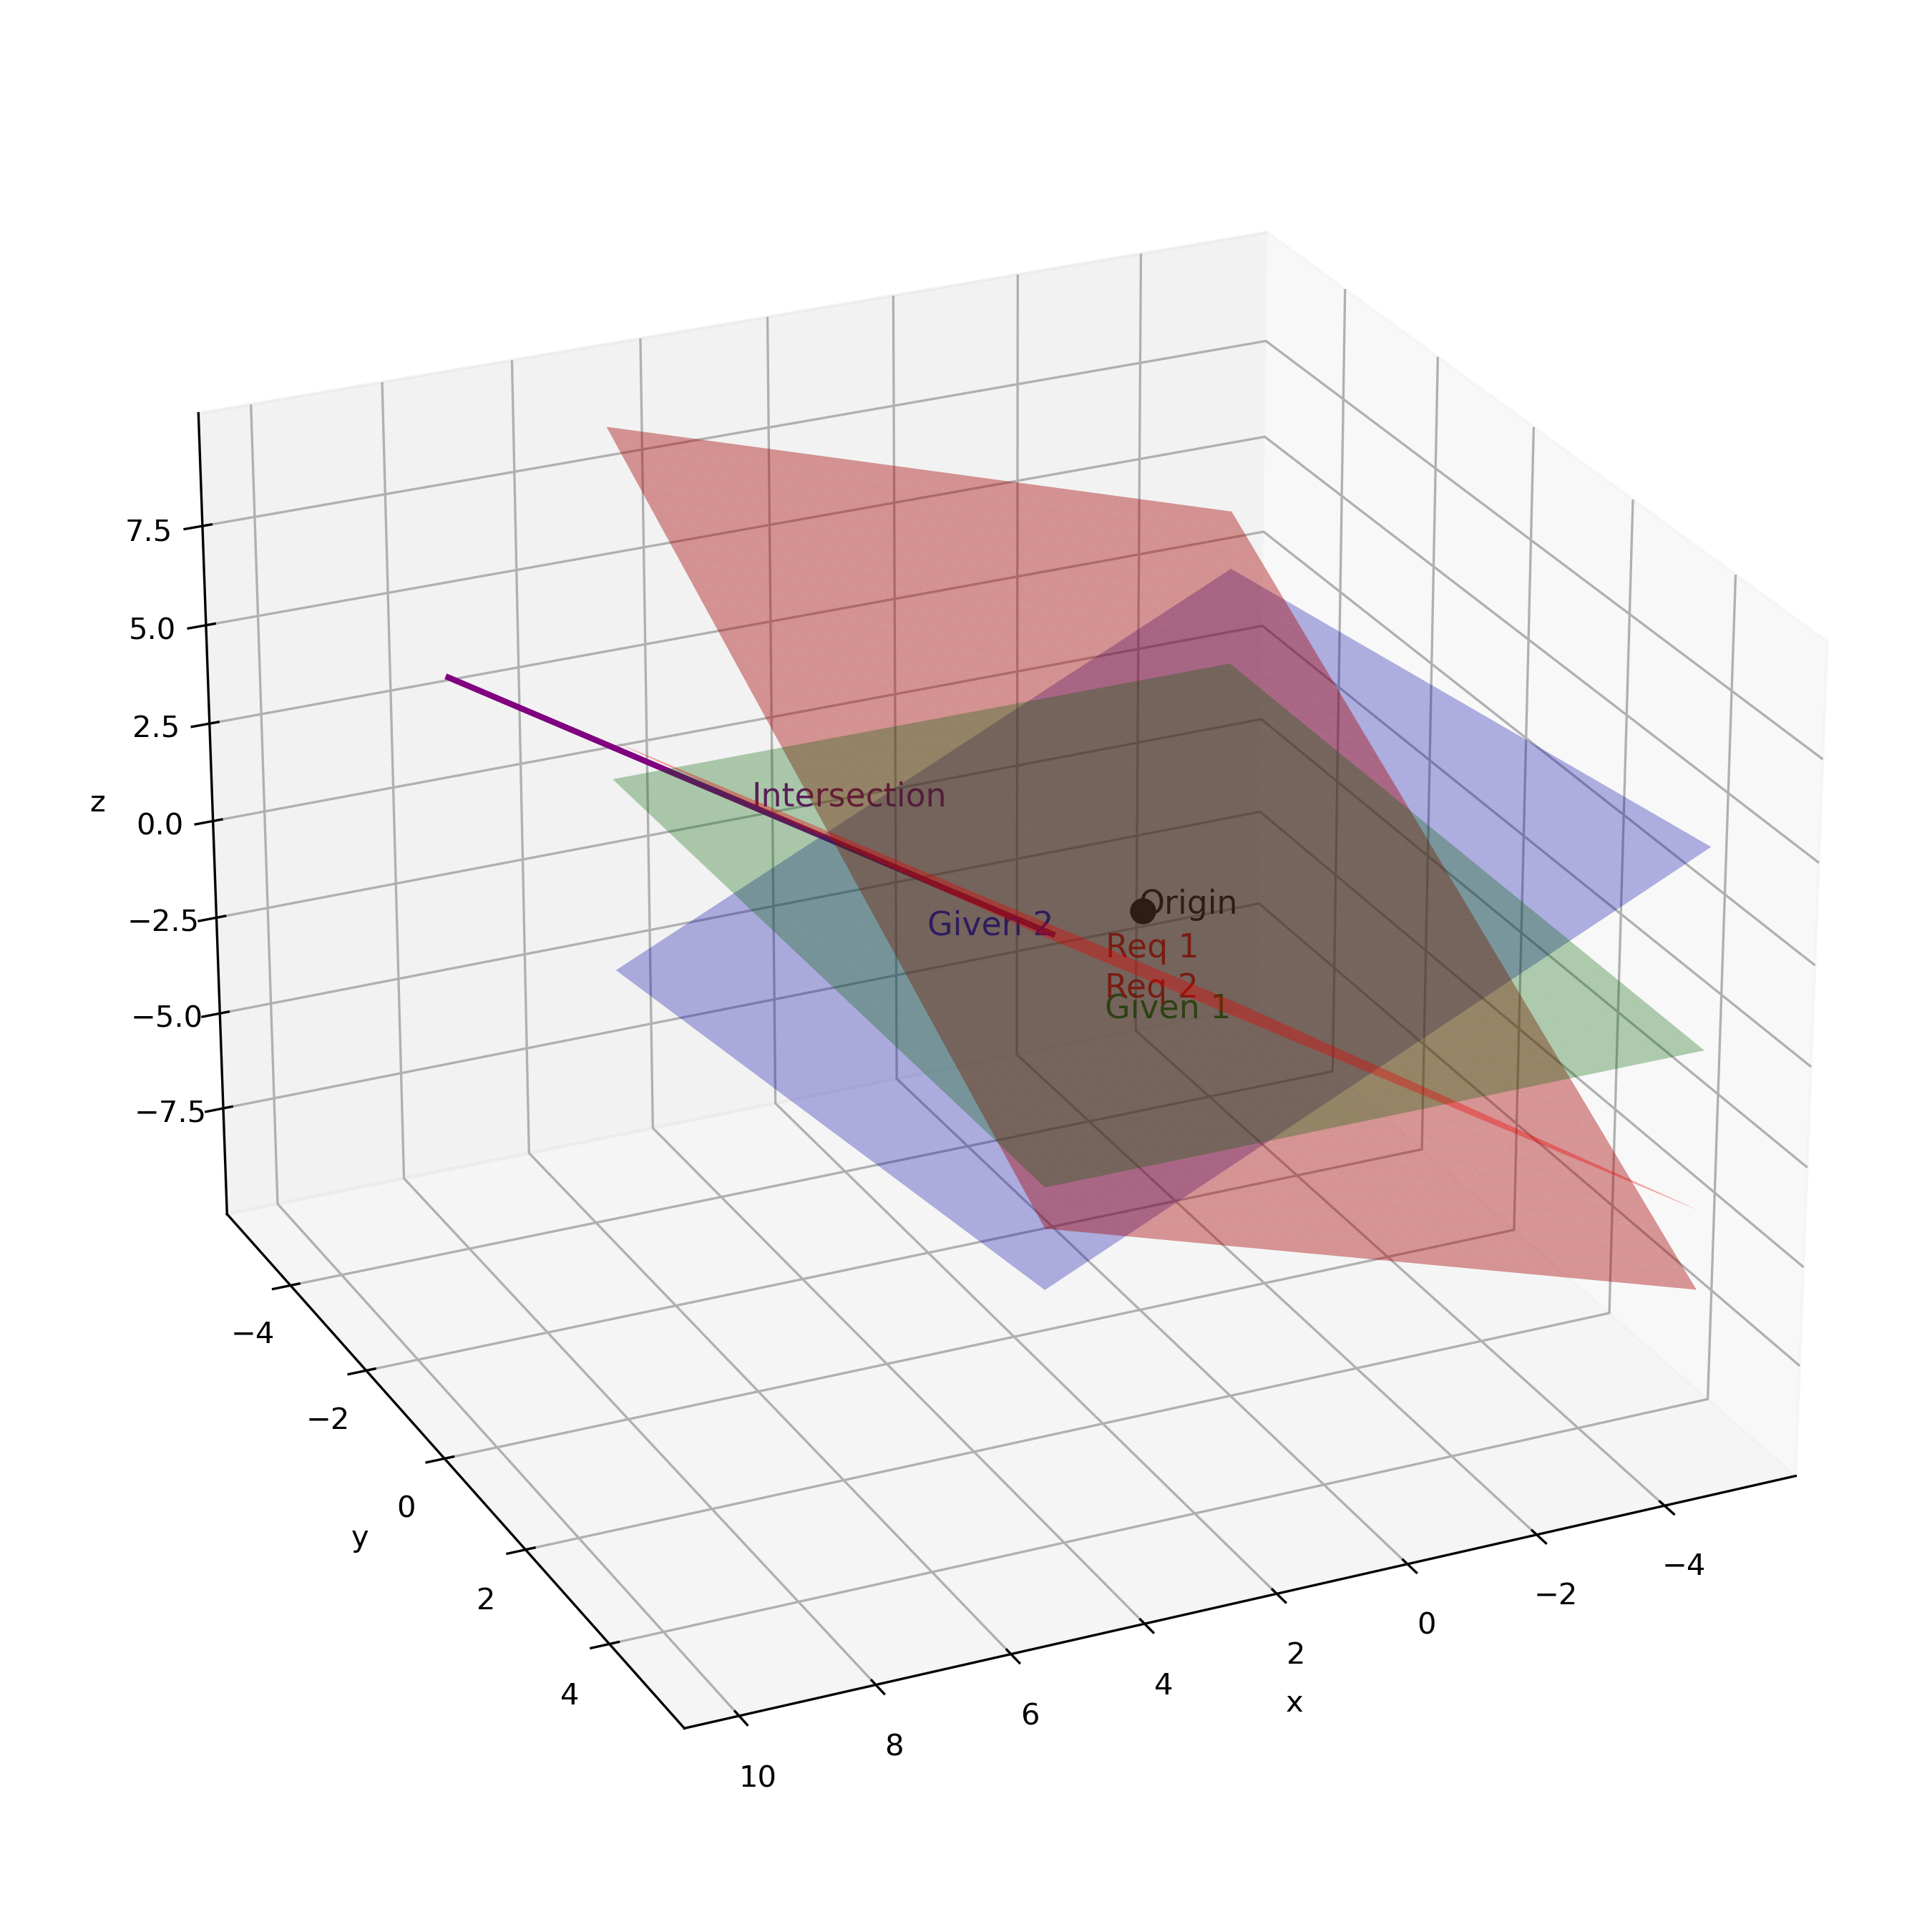
\includegraphics[scale=0.5]{img1}
	\caption*{}
	\label{img1}
\end{figure}
Plot using Python:
\begin{figure}[H]
	\centering
	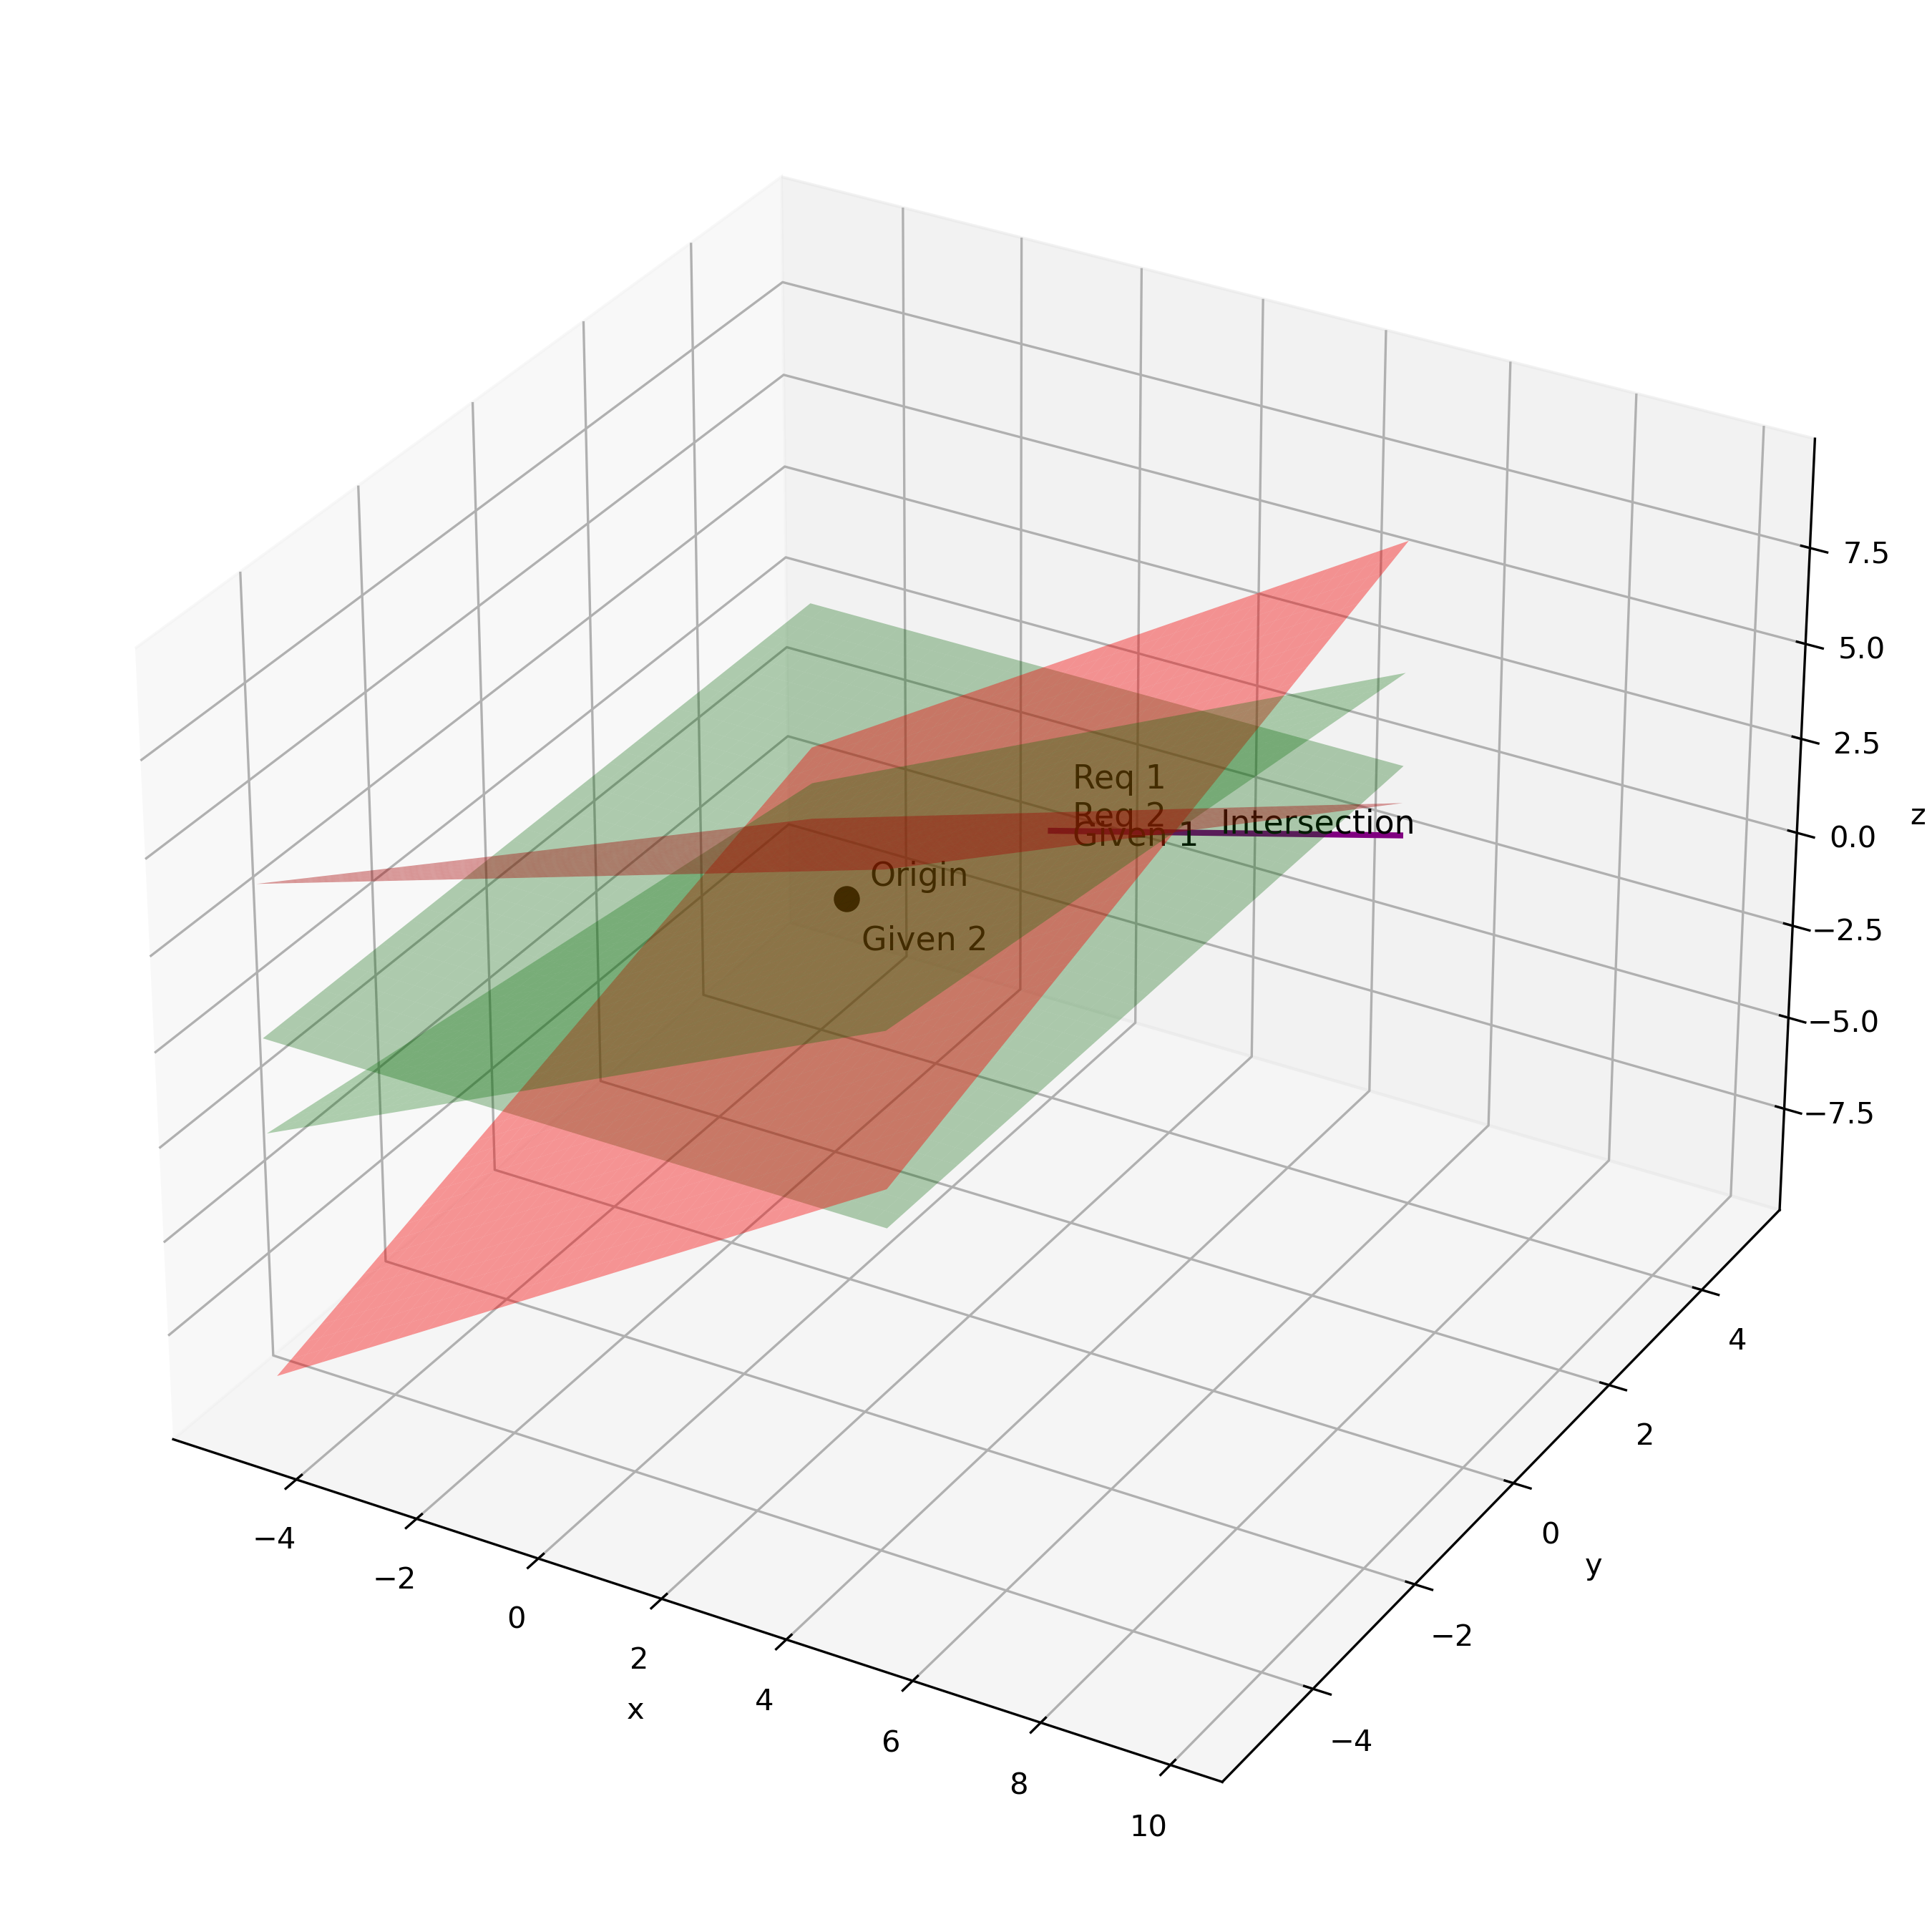
\includegraphics[scale=0.5]{img2}
	\caption*{}
	\label{img2}
\end{figure}
\end{document}

